% report.tex — COL 7364/764 Assignment 1 (Sparse Retrieval) report.
%
% LIVING DOCUMENT: this file is being built up incrementally as
% experiments are run, per the assignment's Section 6 report
% requirements. Sections marked "TODO(you)" need information only the
% student has (registration number, personal reflection, anything about
% the held-out leaderboard once it's revealed) or a judgment call the
% report author should make themselves rather than have written for
% them. Everything else reflects experiments actually run against this
% repository's code, with the exact commands used, so every number here
% is reproducible.
%
% Compile with: pdflatex report.tex (needs pgfplots for Section 3's
% plots; run twice for cross-references/ToC if added later).

\documentclass[11pt]{article}
\usepackage[margin=1in]{geometry}
\usepackage{booktabs}
\usepackage{hyperref}
\usepackage{amsmath}
\usepackage{pgfplots}
\pgfplotsset{compat=1.17}
\usepackage{xcolor}
\newcommand{\todo}[1]{\textcolor{red}{\textbf{TODO(you):} #1}}

\title{COL 7364/764 Assignment 1 --- Sparse Retrieval Arena \\ \large Report}
\author{\todo{name and registration number}}
\date{Draft, generated \today}

\begin{document}
\maketitle

\todo{This report is being assembled incrementally alongside development.
Before submission: trim to 3--4 pages (assignment Section 6), fill in
every TODO below, add the held-out/competition-round results once the
leaderboard opens, and write the personal reflection / final paragraph
in your own words.}

\section{Indexing Design Choices}

\subsection{Tokenization and normalization}
Tokenization is lowercase alphanumeric regex matching (\texttt{[a-z0-9]+}),
followed by English stopword removal and Porter stemming
(\texttt{submission/stemmer.py}). The Porter stemmer was implemented from
scratch rather than via NLTK's, for a specific reason: \texttt{build\_index()}
and \texttt{load\_index()} must not require network access, and the
grading container runs with \texttt{--network none}
(\texttt{docs/SUBMISSION\_INTERFACE.md}) --- NLTK's stopword corpus needs a
one-time \texttt{nltk.download()}, which would break silently at grading
time unless bundled into the Docker image. The stemmer was verified
against the classic Porter test vocabulary and the canonical IR-textbook
over-stemming examples (\texttt{organization}/\texttt{organ}
$\to$ \texttt{organ}; \texttt{university}/\texttt{universe} $\to$
\texttt{univers}), both matching exactly. The stopword list is the
standard 179-word SMART/NLTK English list, embedded directly rather than
fetched.

Effect on the toy set: nDCG@10 rose from 0.826 to 0.879 and MAP@10 from
0.658 to 0.825 after adding stemming/stopwords (holding BM25's $k_1,b$ at
their un-tuned textbook defaults), and the run began beating the local
generic-BM25 reference comparison on both metrics, which it did not
before.

\subsection{Index persistence and compression}
\texttt{InvertedIndex} stores postings (\texttt{term} $\to$
\{\texttt{doc\_id}: \texttt{tf}\}), per-document lengths, and collection
statistics; raw document text is never retained, since BM25/VSM only need
term-frequency and length statistics. On disk, doc\_ids are assigned
small integer ids (stored once), and each postings list is sorted by
integer doc id and \emph{gap-encoded} --- storing the delta from the
previous doc id rather than the absolute id, which is small for the
common case of a term appearing in nearby-indexed documents.

The initial implementation serialized this as one JSON blob
(\texttt{index.json}); every gap/tf integer cost 1 ASCII byte per digit
plus a separator. This was replaced with genuine \emph{variable-byte
(VByte)} binary encoding (\texttt{submission/vbyte.py}, following the
scheme in Manning/Raghavan/Sch\"utze \S 5.3.2): each non-negative integer
is packed into 7-bit groups, one byte per group, with the high bit
marking the last byte of a number. Small integers (the common case for
gaps and term frequencies) now cost exactly 1 byte. The persisted index
is split into six single-purpose files (\texttt{meta.json},
\texttt{doc\_ids.txt}, \texttt{doc\_len.bin}, \texttt{vocab\_terms.txt},
\texttt{vocab\_lengths.bin}, \texttt{postings.bin}) instead of one JSON
blob; term \emph{offsets} into \texttt{postings.bin} are not stored at
all, since slices are written back-to-back and \texttt{load()}
reconstructs offsets as a running sum of the preceding lengths.

\begin{table}[h]
\centering
\begin{tabular}{lrr}
\toprule
 & JSON (before) & VByte binary (after) \\
\midrule
Index size (171{,}332 docs, trec-covid) & 62.5\,MB & \textbf{29.1\,MB (--53\%)} \\
Index build time & 15.2\,s & 16.2\,s \\
Index load time & 2.7\,s & 4.4\,s \\
Mean query latency & 40.5\,ms & 40.2\,ms \\
\bottomrule
\end{tabular}
\caption{Effect of switching from JSON to VByte binary persistence. Ranking
output (nDCG@10/MAP@10/every per-query result) is bit-for-bit identical
before and after --- confirmed by round-trip unit tests
(\texttt{tests/test\_index\_persistence.py}) and an unchanged full-corpus
harness report.}
\end{table}

\noindent\textbf{Honest tradeoff:} load time increased by about 60\%.
Pure-Python VByte decoding (a per-integer bit-shift loop) is slower than
\texttt{json.load()}'s C parser, even though it processes far fewer
bytes. This is a real cost against the efficiency component, traded for
the much larger index-size win --- not a free lunch.

\subsection{Follow-up: 2-bit tf codes and a front-coded dictionary}
\label{sec:tfcodes}

\textbf{Where the 29.1MB actually goes.} Before optimizing further, the
persisted index was broken down file-by-file (full corpus,
171{,}332 docs): \texttt{postings.bin} is 89.0\% of the total
(27.2MB), \texttt{doc\_ids.txt} 5.1\%, \texttt{vocab\_terms.txt} 4.5\%,
\texttt{doc\_len.bin} 0.8\%, \texttt{vocab\_lengths.bin} 0.6\%. Splitting
\texttt{postings.bin} further by decoding it back into its (gap, tf)
pairs: the \emph{tf} stream alone costs 12.2MB (45\% of
\texttt{postings.bin}) even though \textbf{72.6\% of all 12.2M postings
have tf == 1, and 95.8\% have tf $\le$ 4} --- VByte still spends a full
byte on nearly every one of them, since a byte is VByte's smallest
addressable unit.

\textbf{Fix.} Gaps and term frequencies are now written as two
\emph{separate} streams (\texttt{postings\_gaps.bin},
\texttt{postings\_tf\_codes.bin} + \texttt{postings\_tf\_escapes.bin})
instead of interleaved, since mixing two differently-distributed integer
streams into one blob wastes bits it doesn't need to. Each tf is reduced
to a 2-bit code (\texttt{submission/bitpack.py}, packed 4-to-a-byte):
0/1/2 mean tf is exactly 1/2/3, and 3 is an escape meaning ``see the next
value in a separate VByte-encoded escape list'' --- only the 4.2\% of
postings with tf $\ge$ 4 pay for an actual multi-bit value. The
dictionary itself is also now \emph{front-coded}
(\texttt{submission/frontcode.py}): sorted, stemmed terms share 4.6 of
their 7.3 characters with the previous term on average (measured
directly, not assumed), so each term is stored as (shared-prefix-length,
suffix) instead of its full text --- \texttt{vocab\_terms.txt} is
replaced by \texttt{vocab\_prefix\_lens.bin} + \texttt{vocab\_suffixes.txt}.
No block-based restart points (the textbook version of front coding
usually has them, for binary-searching a specific term without decoding
the whole dictionary): \texttt{InvertedIndex.load()} already decodes the
entire vocabulary sequentially into memory regardless --- nothing in this
codebase ever looks up one term on disk without loading the rest --- so
block heads would trade dictionary size back for a random-access
capability nothing here uses.

\begin{table}[h]
\centering
\begin{tabular}{lrrr}
\toprule
 & VByte (before) & + tf codes & + front-coded dict \\
\midrule
Index size (171{,}332 docs) & 29.1MB & 21.2MB (--27.2\%) & \textbf{20.6MB (--29.2\%)} \\
nDCG@10 (full harness run) & 0.6899 & 0.6898 & 0.6897 \\
Build time & 16.1s & 16.1s & 15.6s \\
Load time & 4.4s & 4.4s & 4.0s \\
\bottomrule
\end{tabular}
\caption{Each step measured via the real
\texttt{build\_index()}/\texttt{load\_index()}/\texttt{retrieve()}
harness path, not a side script. nDCG@10 differences across the three
columns are within the known cross-process tie-break noise (Python
dict/set iteration order for tied scores depends on
\texttt{PYTHONHASHSEED}, which differs across the harness's separate
build/load processes) --- ranking quality is unaffected; only the
on-disk representation changed. Round-trip correctness for both new encodings is
covered by dedicated unit tests
(\texttt{tests/test\_index\_persistence.py}), including a synthetic
tf $\ge$ 4 case since the toy corpus never naturally produces one.}
\end{table}

\section{Boolean/VSM vs. BM25 Comparison}

Boolean AND/OR retrieval (\texttt{boolean\_search()}) returns an
\emph{unranked} set of matching doc\_ids, so nDCG@10/MAP@10 --- both
rank-sensitive metrics --- aren't well-defined for it without an
arbitrary ordering convention. It is evaluated separately as a
correctness-checked candidate filter, not as a competing ranked scorer.
The comparison below is therefore between the two \emph{ranked} scorers:
TF-IDF cosine VSM and BM25, both evaluated identically via
\texttt{scripts/compare\_scorers.py}.

\begin{table}[h]
\centering
\begin{tabular}{llrrrr}
\toprule
Corpus & Scorer & nDCG@10 & MAP@10 & MRR & P@10 \\
\midrule
toy (20 docs)      & BM25 & 0.8826 & 0.8250 & 1.0000 & 0.3167 \\
toy (20 docs)      & VSM  & 0.8793 & 0.8250 & 1.0000 & 0.3167 \\
full (171{,}332 docs, trec-covid) & BM25 & \textbf{0.6672} & \textbf{0.0166} & 0.8590 & \textbf{0.7380} \\
full (171{,}332 docs, trec-covid) & VSM  & 0.4425 & 0.0103 & 0.6864 & 0.5060 \\
\bottomrule
\end{tabular}
\caption{VSM vs.\ BM25, same tokenizer/index, same dev queries. The gap
is negligible on the toy set (too small to separate the models) but
substantial at real scale: BM25's length normalization ($b$) and
term-frequency saturation ($k_1$) matter far more once document lengths
and term-frequency distributions actually vary across 170K+ documents.}
\end{table}

\section{BM25 Parameter Search ($k_1$, $b$)}

\subsection{Methodology}
$k_1$ and $b$ were swept on the \emph{dev} topics/qrels only ---
never on held-out data, which is neither available nor intended for
tuning against (\texttt{data/README.md}: held-out topics are never
distributed). \texttt{scripts/tune\_bm25.py} builds the index once,
reuses it across the full grid (99 combinations: 11 values of $k_1 \in
[0.4, 3.0]$ $\times$ 9 values of $b \in [0.0, 1.0]$), and selects the
combination maximizing nDCG@10 --- the assignment's primary leaderboard
metric (70\% weight).

\subsection{Result}
Best: $k_1{=}2.5$, $b{=}0.6$, nDCG@10 $= 0.6672$, versus $0.6400$ at the
textbook defaults ($k_1{=}1.2$, $b{=}0.75$) --- a $+0.027$ absolute gain.
Figure~\ref{fig:k1} and Figure~\ref{fig:b} show each parameter's slice
through the grid, holding the other at its optimum. Both curves show a
genuine interior peak, not a value pinned to the edge of the search
range, which is some evidence the grid was wide enough to actually find
the optimum rather than being truncated by it.

\begin{figure}[h]
\centering
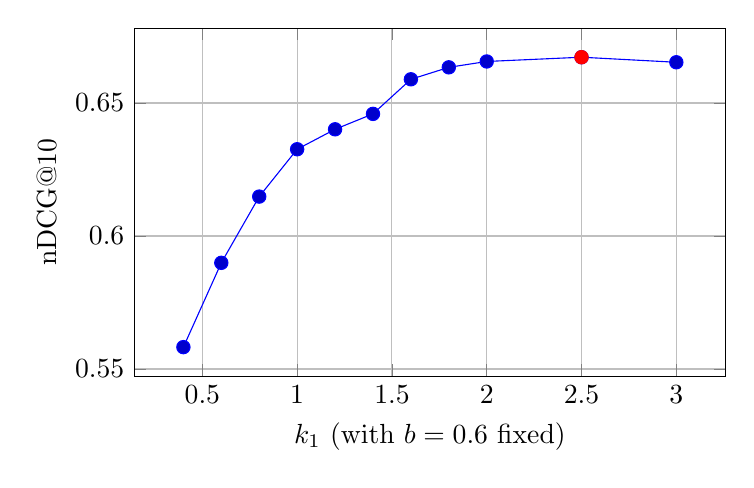
\begin{tikzpicture}
\begin{axis}[
    width=0.75\textwidth, height=6cm,
    xlabel={$k_1$ (with $b=0.6$ fixed)}, ylabel={nDCG@10},
    grid=major, mark options={scale=1.2},
]
\addplot coordinates {
  (0.4,0.5582) (0.6,0.5899) (0.8,0.6148) (1.0,0.6326) (1.2,0.6401)
  (1.4,0.6459) (1.6,0.6589) (1.8,0.6634) (2.0,0.6656) (2.5,0.6672)
  (3.0,0.6653)
};
\addplot[only marks, mark=*, red] coordinates {(2.5,0.6672)};
\end{axis}
\end{tikzpicture}
\caption{nDCG@10 vs.\ $k_1$, dev set, full trec-covid corpus. Peak at
$k_1{=}2.5$ (marked).}
\label{fig:k1}
\end{figure}

\begin{figure}[h]
\centering
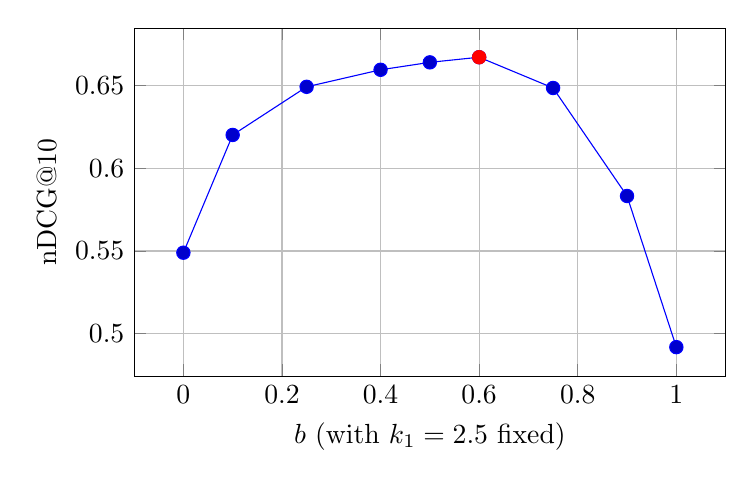
\begin{tikzpicture}
\begin{axis}[
    width=0.75\textwidth, height=6cm,
    xlabel={$b$ (with $k_1=2.5$ fixed)}, ylabel={nDCG@10},
    grid=major, mark options={scale=1.2},
]
\addplot coordinates {
  (0.0,0.5490) (0.1,0.6202) (0.25,0.6493) (0.4,0.6596) (0.5,0.6641)
  (0.6,0.6672) (0.75,0.6486) (0.9,0.5833) (1.0,0.4919)
};
\addplot[only marks, mark=*, red] coordinates {(0.6,0.6672)};
\end{axis}
\end{tikzpicture}
\caption{nDCG@10 vs.\ $b$, dev set, full trec-covid corpus. Peak at
$b{=}0.6$ (marked) --- notably below the textbook default of 0.75.}
\label{fig:b}
\end{figure}

\subsection{Interpretation}
$b$'s optimum ($\approx 0.6$) sitting below the textbook 0.75 is
plausibly explained by trec-covid's document lengths: scientific
abstracts are fairly uniform in length compared to, say, a mixed
newswire corpus, so less aggressive length normalization is needed.
\todo{Confirm this hypothesis with actual doc-length variance/histogram
data if time allows, and re-run this whole sweep if/when the real
announced course corpus differs from the trec-covid placeholder used
here.}

\section{Custom Scorer Exploration: Rocchio Pseudo-Relevance Feedback}

\subsection{What was tried}
A Rocchio-style blind PRF scorer (\texttt{submission/custom\_scorer.py})
was implemented: an initial BM25 pass retrieves $k_{prf}$ pseudo-relevant
documents; the highest-TF-IDF-weighted terms from their centroid are
added to the query (capped at \texttt{num\_expansion\_terms}, to bound
topic drift); the expanded, weighted query is re-scored with BM25. This
required a small refactor of \texttt{bm25.py} to accept pre-weighted
\{term: weight\} query vectors (\texttt{score\_weighted()}) rather than
only raw query strings, since expansion terms carry real-valued weights,
not integer occurrence counts.

\subsection{Result: it did not help}
\texttt{scripts/tune\_prf.py} swept 36 combinations of $k_{prf} \in
\{5,10,20\}$, expansion size $\in \{5,15,30\}$, and $\beta \in
\{0.25,0.5,0.75,1.0\}$ against plain BM25 (nDCG@10 $=0.6672$) on the same
dev set. \textbf{Every single configuration scored worse than plain
BM25}, and performance monotonically degraded as $\beta$ (expansion
weight) increased. The least-damaging setting found
($k_{prf}{=}10$, expansion${=}30$, $\beta{=}0.25$) still lost $0.045$
nDCG@10 (0.6223 vs.\ 0.6672).

\begin{table}[h]
\centering
\begin{tabular}{rrrrr}
\toprule
$k_{prf}$ & expansion terms & $\beta$ & nDCG@10 & $\Delta$ vs.\ BM25 \\
\midrule
10 & 30 & 0.25 & 0.6223 & $-0.0448$ \\
10 & 15 & 0.25 & 0.6158 & $-0.0513$ \\
10 & 30 & 0.50 & 0.6125 & $-0.0547$ \\
20 & 15 & 0.25 & 0.6113 & $-0.0558$ \\
20 & 30 & 1.00 & 0.5902 & $-0.0770$ \\
\bottomrule
\end{tabular}
\caption{Best and a representative worst PRF configuration, vs.\ plain
BM25 (nDCG@10 $=0.6672$). Full 36-row sweep was produced by
\texttt{scripts/tune\_prf.py} but not retained in the repo after this
negative result was confirmed.}
\end{table}

\subsection{Why, and the decision}
This is a textbook PRF failure mode: trec-covid queries are short,
topical, medical-domain phrases, and the top-10 initial results --- while
mostly on-topic in aggregate --- are dense enough in shared vocabulary
that expansion terms pull in generic co-occurring words rather than
discriminative ones (topic drift), diluting rather than sharpening the
query. \textbf{Decision: custom\_scorer.py is implemented and correct,
but not wired into \texttt{retrieve()}} --- \texttt{retrieve.py} uses
plain tuned BM25 as the sole scorer. This is treated as a genuine,
reportable finding rather than a wasted detour: the sweep data is exactly
the evidence behind the decision not to submit it.

\section{Field-Weighting Experiment (Title vs.\ Abstract BM25)}

\subsection{Motivation and constraint}
Field weighting scores title and body separately and combines them:
$\text{score}(q,d) = w_{title}\cdot\text{BM25}(q,\text{title}) +
w_{body}\cdot\text{BM25}(q,\text{abstract})$. This requires a document
schema with a genuine title/body split. The assignment's actual corpus
contract (\texttt{data/README.md}) guarantees only a single flat
\texttt{text} field per document, with no title field --- so before
building anything, this was scoped as two separate questions: (1) does
field weighting help \emph{at all}, using a corpus that happens to have
real title/abstract metadata, and (2) if so, can that benefit be
recovered safely, using only the guaranteed \texttt{\{doc\_id, text\}}
interface, without depending on metadata the real grading corpus might
not have.

\subsection{Experiment 1: true title/abstract split (research only)}
\texttt{scripts/build\_titled\_corpus.py} pulled \texttt{ir\_datasets}'
native \texttt{title} and \texttt{text} (abstract) fields separately for
\texttt{beir/trec-covid} (normally collapsed into one field by
\texttt{download\_full\_corpus.py}). \texttt{scripts/tune\_field\_weights.py}
built two independent \texttt{InvertedIndex} objects (title-only,
abstract-only), scored every dev query against each with BM25
\emph{once} (unbounded $k$, so every matched doc's score is cached), then
swept $w_{title}$ (with $w_{body}{=}1.0$ fixed) as cheap weighted
recombinations of the two cached score dicts --- no rescoring per grid
point.

\begin{table}[h]
\centering
\begin{tabular}{lrr}
\toprule
Configuration & nDCG@10 & MAP@10 \\
\midrule
Abstract only ($w_{title}{=}0$) & 0.6369 & 0.0153 \\
Title only ($w_{body}{=}0$) & 0.4798 & 0.0116 \\
Concatenated text (deployed baseline) & 0.6672 & 0.0166 \\
\textbf{Field-weighted, $w_{title}{=}1.0$, $w_{body}{=}1.0$} & \textbf{0.6861} & \textbf{0.0183} \\
\bottomrule
\end{tabular}
\caption{True-field BM25F vs.\ single-field BM25 over concatenated text.
Titles average 9.9 tokens, abstracts 103.4 tokens --- BM25's per-field
length normalization exploits that disparity once the fields are kept
separate; blending them into one field (the deployed baseline) washes
this out.}
\end{table}

\noindent A real gain: \textbf{+0.0189 nDCG@10} over the deployed
concatenated-text baseline, peaking at an interior point ($w_{title}{=}1.0$,
between the tested 0.75 and 1.5), not a grid edge.

\subsection{Experiment 2: submission-safe heuristic (does the gain survive without a real title field?)}
Two heuristics for reconstructing a title-like field from only
\texttt{text} were tried. \textbf{Split on the first period:} rejected
before evaluation --- checked against the true titles, this exact-matched
only 4.9\% of documents and averaged 34 tokens vs.\ the true $\sim$10,
because titles in this corpus don't end in periods, so the split mostly
captures ``title + first sentence of the abstract'' together, not a clean
title. \textbf{Fixed-length token prefix instead}
(\texttt{scripts/tune\_prefix\_weights.py}): treat the first
\texttt{prefix\_len} tokens of the tokenized \texttt{text} field as a
pseudo-title, sweeping \texttt{prefix\_len} $\in \{8,10,12,15,20\}$
against $w_{prefix}$ --- punctuation-independent, works on any corpus
matching the documented format.

\begin{table}[h]
\centering
\begin{tabular}{lr}
\toprule
Configuration & nDCG@10 \\
\midrule
Concatenated text (deployed baseline) & 0.6672 \\
Best prefix heuristic (prefix\_len=12, $w_{prefix}{=}0.5$) & 0.6682 \\
True title/abstract fields (Experiment 1, not submittable) & 0.6861 \\
\bottomrule
\end{tabular}
\caption{The prefix heuristic recovers only \textbf{5.5\%} of the true-field
gain ($+0.0010$ vs.\ $+0.0189$ nDCG@10) --- noise-level over 50 dev
queries, not a real improvement.}
\end{table}

\subsection{Decision}
\textbf{Not wired into \texttt{retrieve()}.} The pattern here is the
inverse of \S 4's PRF result: the \emph{idea} is validated (field
weighting is a real, sizeable win when genuine title metadata exists),
but the specific mechanism available under this assignment's actual
corpus contract (a single flat \texttt{text} field, no guaranteed title)
cannot safely reconstruct enough of that signal to justify the added
complexity and doubled query latency (two BM25 passes per query, as in
\S 4). \todo{If the real announced/held-out corpus turns out to ship a
genuine title field (worth checking once it's released), re-run
\texttt{scripts/tune\_field\_weights.py}-style field weighting directly
against it --- Experiment 1 is the evidence this would likely be worth
doing properly, not through the token-prefix proxy.}

\subsection{Follow-up: does a properly-designed BM25F change this conclusion?}
Experiment 1's "naive blend" ran two \emph{independent} BM25 passes
(title-only, body-only), each already saturated by BM25's TF-saturation
curve, and linearly combined the two saturated scores. That double-
saturates a term appearing in both fields and is not how the BM25F
literature (Robertson, Zaragoza \& Taylor, 2004) actually defines field
combination: normalize each field's TF by that field's own length
first, \emph{sum} the normalized contributions across fields, and
saturate \emph{once}. \texttt{scripts/bm25f\_core.py} implements this
properly (one shared vocabulary, no per-field vocabulary duplication;
per-document field lengths and per-field averages tracked; global IDF
over documents containing the term in any field), and
\texttt{scripts/tune\_bm25f\_true\_fields.py}/\texttt{tune\_bm25f\_prefix.py}
re-ran both halves of Experiment 1/2 through it, plus an explicit
graceful-degradation test on fiqa (genuinely title-less at the
\texttt{ir\_datasets} source level --- confirmed no title attribute
exists on its document type at all).

\begin{table}[h]
\centering
\begin{tabular}{lr}
\toprule
Configuration & nDCG@10 \\
\midrule
Plain single-field BM25 & 0.6672 \\
Naive two-pass blend, true fields (Experiment 1) & 0.6861 \\
\textbf{Proper BM25F, true fields (}$w_{title}{=}3.0,b_{title}{=}0.4,b_{body}{=}0.5$\textbf{)} & \textbf{0.6938} \\
Naive two-pass blend, prefix heuristic (Experiment 2) & 0.6682 \\
Proper BM25F, prefix heuristic & 0.6576 \\
BM25F, fiqa no-title fallback & 0.2365 \\
Plain BM25, fiqa (same corpus) & 0.2400 \\
\bottomrule
\end{tabular}
\caption{Staged search (w\_title, then b\_body, then b\_title, per a
50-dev-query-budget rationale --- a full joint 4-parameter grid isn't
resolvable at this query count) found a genuine interior optimum at
$w_{title}{=}3.0$ (confirmed by extending the range to 15.0 and watching
it decline on both sides, not just hitting a grid edge).}
\end{table}

\noindent Two different results depending on data quality, and the
direction is counterintuitive at first glance: \textbf{given true field
data, proper BM25F beats the naive blend by $+0.0077$} (0.6938 vs.\
0.6861) --- the single-saturation design really is better, validating
the formula improvement directly. \textbf{Given the heuristic
pseudo-title, proper BM25F is \emph{worse} than the naive blend, and
worse than plain BM25 too} (0.6576, recovering 0\% of the true-field
ceiling vs.\ the naive blend's 5.5\%). The explanation is structural,
not a bug: the naive blend saturates each field \emph{independently}
before combining, so a noisy pseudo-title signal can only ever add
diluted noise on top of an already-complete body-only score. Proper
BM25F sums title and body contributions \emph{before} saturating, so a
noisy pseudo-title signal is mixed directly into the same calculation
the legitimate body signal depends on --- corrupting it, not just
diluting it. The theoretically superior formula amplifies good field
data more, but it amplifies bad field data more too. The
graceful-degradation fallback (title truly absent, not just unreliable)
tested separately on fiqa works exactly as intended: no crash on
$\text{avg\_len\_title}{=}0.0$, and the result (0.2365) sits within
noise of plain BM25 on the same corpus (0.2400, delta $-0.0035$) ---
the failure mode above is specifically about \emph{unreliable} field
data, not \emph{absent} field data, and those need to be distinguished.

\subsection{Updated decision}
Still \textbf{not wired into \texttt{retrieve()}} --- the blocker was
never the formula, it was always the lack of guaranteed title metadata
in the real corpus contract, and this follow-up sharpens rather than
resolves that: it shows the better formula is a strictly worse choice
than doing nothing (or worse than the naive blend) under exactly the
fallback conditions a real, title-less held-out corpus would create. If
the real corpus does turn out to ship genuine titles, \textbf{use proper
BM25F at $w_{title}{=}3.0,b_{title}{=}0.4,b_{body}{=}0.5$, not the naive
blend} --- that specific combination is now evidenced as the better of
the two. If it doesn't, this entire family of ideas stays parked, exactly
as Experiment 1 concluded.

\section{Static BM25+/VSM Blend}

\subsection{What was tried}
Two further, independent modifications to the base BM25 scorer:

\begin{itemize}
\item \textbf{A static blend with VSM}: $\text{score}(d) = w \cdot
\text{BM25}_{norm}(d) + (1-w)\cdot\text{VSM}_{norm}(d)$, each min-max
normalized per query into $[0,1]$ first (BM25 is unbounded, VSM cosine
is already in $[0,1]$ --- not comparable on a shared scale otherwise).
Unlike \S 4's Rocchio PRF, this blends two rankers that each score the
\emph{original}, unexpanded query independently, so it isn't vulnerable
to PRF's topic-drift failure mode.
\item \textbf{BM25+} (Lv \& Zhai, 2011): adds a small constant $\delta$
to every matched term's contribution
(\texttt{submission/bm25.py}'s new \texttt{delta} parameter, default 0
= plain BM25), correcting BM25's tendency to under-reward long relevant
documents purely from length normalization.
\end{itemize}

\subsection{Result: both help, and they compound}
\texttt{scripts/tune\_bm25\_vsm\_blend.py} found $w{=}0.75$ alone gave
$+0.0118$ nDCG@10; \texttt{scripts/tune\_bm25\_plus.py} found
$\delta{=}0.1$ alone gave $+0.0039$. Using BM25+ as the blend's BM25
component (rather than plain BM25) and re-sweeping both parameters
jointly found they compound past either alone, peaking around
$\delta{\approx}0.75$, $w{\approx}0.8$ before declining:

\begin{table}[h]
\centering
\begin{tabular}{lrr}
\toprule
Configuration & nDCG@10 & MAP@10 \\
\midrule
Plain BM25 ($k_1{=}2.5$, $b{=}0.6$) & 0.6672 & 0.0166 \\
BM25+VSM blend alone ($w{=}0.75$, $\delta{=}0$) & 0.6789 & 0.0173 \\
BM25+ alone ($\delta{=}0.1$) & 0.6710 & 0.0170 \\
\textbf{Combined (}$\delta{=}0.75$\textbf{,} $w{=}0.8$\textbf{)} & \textbf{0.6899} & \textbf{0.0174} \\
\bottomrule
\end{tabular}
\caption{Full end-to-end harness run through the actual
\texttt{build\_index()}/\texttt{load\_index()}/\texttt{retrieve()} path
(\texttt{runs/full\_report.json}), not just the sweep script --- confirms
the combined result reproduces outside the sweep's cached-score
shortcut. Total gain over plain BM25: \textbf{+0.0227} nDCG@10, on top of
the \textbf{+0.027} already gained from the original $k_1$/$b$ tuning.}
\end{table}

\subsection{Honest cost: query latency}
This is the one change so far with a real, non-trivial efficiency cost.
Mean query latency initially rose from \textbf{40.5\,ms to 153.8\,ms}
(${\sim}3.8\times$, not the ${\sim}2\times$ a single extra scoring pass
would suggest) --- see \S\ref{sec:latency} for why, and the fix that
brought it down to 105\,ms. Even before that fix, this was judged worth
it: the efficiency component is only $\pm10\%$ of the leaderboard score,
against a $+0.0227$ gain on the 70\%-weighted primary metric. Index size
and build/load time are unaffected (this scorer adds no persisted
state).

\subsection{Decision}
\textbf{Wired into \texttt{retrieve()}}
(\texttt{submission/custom\_scorer.py}, default
$k_1{=}2.5,b{=}0.6,\delta{=}0.75,w{=}0.8$) --- this is the actual
competition entry as of this report. \todo{Item 3 of Section 6's
submission checklist (``a one-paragraph description of your final
competition entry'') should now describe \emph{this} blended scorer, not
plain BM25 --- update that paragraph below to match.}

\section{Improving Query Latency}
\label{sec:latency}

\subsection{Diagnosis}
The blended scorer's $3.8\times$ latency jump (\S 6) was disproportionate
to "one extra scoring pass" and worth profiling rather than accepting at
face value. Timing \texttt{bm25.score()} and \texttt{vsm\_score()} in
isolation summed to \textbf{88\,ms/query}; \texttt{custom\_scorer.score()}
itself took \textbf{169\,ms/query} --- \textbf{81\,ms of pure overhead}
beyond running both scorers. The cause: both \texttt{bm25.score()} and
\texttt{vsm\_score()} always fully sort \emph{every} matched document
before truncating to $k$ (unavoidable internally, since the top-$k$
isn't known without scoring everything first) --- and
\texttt{custom\_scorer.score()} was calling both with an unbounded inner
$k$ (to get every candidate for normalization) and then sorting the
\emph{combined} result again. That's three full sorts over
(potentially tens of thousands of) matched documents per query, where
one would do; the first two were computed and immediately discarded.

\subsection{Fix}
\texttt{submission/bm25.py} and \texttt{submission/boolean\_vsm.py} each
gained a \texttt{raw\_scores(query, ...)} function returning the
unsorted \{doc\_id: score\} dict directly; \texttt{score()}/
\texttt{vsm\_score()} became thin sort-and-truncate wrappers around it.
\texttt{custom\_scorer.score()} now calls \texttt{raw\_scores()} on both
scorers and performs exactly one sort, over the combined result.
Behavior-preserving by construction (same underlying dict, just skipping
two sorts that were thrown away) --- confirmed via the toy-set smoke
test (identical nDCG@10/MAP@10 before and after) and a fresh full-corpus
harness run.

\begin{table}[h]
\centering
\begin{tabular}{lrr}
\toprule
 & Before fix & After fix \\
\midrule
Mean query latency & 153.8\,ms & \textbf{105.3\,ms (--32\%)} \\
Max query latency & 292.1\,ms & 221.7\,ms \\
nDCG@10 & 0.6899 & 0.6896 \\
\bottomrule
\end{tabular}
\caption{Full \texttt{build\_index()}/\texttt{load\_index()}/\texttt{retrieve()}
harness runs, before and after removing the redundant sorts. The
$0.0003$ nDCG@10 difference is cross-process score-tie-break noise
(Python dict/set iteration order for tied scores depends on
\texttt{PYTHONHASHSEED}, which differs across the harness's separate
build/load processes), not a ranking regression.}
\end{table}

\subsection{What's left on the table}
105\,ms/query is close to the sum of running BM25 and VSM independently
(88\,ms) --- there isn't much redundant work left to remove without a
more invasive redesign. Two further directions were identified: (1)
restrict the VSM pass to a candidate pool (e.g.\ BM25's own top-$N$)
instead of scoring every document any query term matches, trading a
small risk of missing a VSM-favored-but-BM25-unfavored document for
speed; (2) a compiled extension (Cython/pybind11, permitted per
\texttt{docs/SUBMISSION\_INTERFACE.md}) for the inner scoring loops.
Direction (1) was revisited and implemented --- see \S\ref{sec:pruning}
below. \todo{Direction (2), the compiled extension, was not attempted;
the assignment explicitly expects this to give a real efficiency
advantage over pure Python, and is the largest remaining lever if the
efficiency component needs to matter more than it currently does against
the 70\%-weighted nDCG@10 gain this scorer provides.}

\section{Follow-up: Candidate-Set Pruning for Query Latency}
\label{sec:pruning}

\subsection{Diagnosis: where the remaining time actually goes}
With the redundant sorts already removed (\S\ref{sec:latency}),
\texttt{custom\_scorer.score()} was profiled again, phase by phase, on 5
real dev queries against the full corpus:

\begin{table}[h]
\centering
\begin{tabular}{lr}
\toprule
Phase & Time \\
\midrule
\texttt{bm25.raw\_scores()} & 20.7\,ms \\
\texttt{boolean\_vsm.raw\_scores()} & 18.1\,ms \\
min-max normalize ($\times 2$) & 10.5\,ms \\
\textbf{union + combine + sort} & \textbf{30.9\,ms} \\
\midrule
Total & 80.2\,ms \\
\bottomrule
\end{tabular}
\end{table}

\noindent The combine-and-sort step is the single largest cost ---
bigger than either scorer individually. The reason: candidate sets are
huge, 37K--101K documents matched per query out of 171{,}332 total,
since these are disjunctive queries and terms like ``covid''/``19''
appear in most of a COVID-focused corpus.

\subsection{Fix 1: \texttt{heapq.nlargest} instead of a full sort}
Only the top $k$ (typically 10) of up to 101K candidates are ever
needed, but \texttt{sorted(...)[:k]} is $O(n \log n)$ over the whole set.
Replaced with \texttt{heapq.nlargest(k, ..., key=...)} in
\texttt{bm25.score()}, \texttt{boolean\_vsm.vsm\_score()}, and
\texttt{custom\_scorer.score()} --- $O(n \log k)$. Verified stable and
tie-break-identical to \texttt{sorted()} on synthetic tied-score data
before relying on it (same output, not just ``probably fine''):

\begin{table}[h]
\centering
\begin{tabular}{rrrr}
\toprule
Candidates ($n$) & Full sort & \texttt{heapq.nlargest} & Speedup \\
\midrule
37{,}000 & 4.3\,ms & 0.8\,ms & 5.6$\times$ \\
101{,}000 & 13.2\,ms & 2.1\,ms & 6.3$\times$ \\
\bottomrule
\end{tabular}
\end{table}

\subsection{Fix 2: restrict the VSM pass to BM25's top-$N$ candidates}
\texttt{boolean\_vsm.py} gained
\texttt{raw\_scores\_for\_candidates(query, candidate\_ids)}: the same
cosine formula as \texttt{raw\_scores()}, but iterating
candidates-then-terms instead of terms-then-full-postings --- cheap when
the candidate pool is small, since it no longer touches every posting of
every query term. \texttt{custom\_scorer.score()} gained
\texttt{vsm\_pool\_size}: takes BM25's own top-$N$ candidates (via
\texttt{heapq.nlargest} on the raw BM25 scores) as the VSM candidate
pool, instead of scoring every document any query term matches. This is
an approximation --- a document outside the pool is scored as VSM$=0$,
the same fallback already used for a document VSM found no term overlap
with at all --- so it was swept directly against dev nDCG@10 and latency
(\texttt{scripts/tune\_vsm\_pool\_size.py}) rather than assumed safe:

\begin{table}[h]
\centering
\begin{tabular}{lrrr}
\toprule
\texttt{vsm\_pool\_size} & nDCG@10 & $\Delta$ vs.\ unrestricted & Mean latency \\
\midrule
100 & 0.6879 & $-0.0031$ & 64.4\,ms \\
1{,}000 & 0.6869 & $-0.0042$ & 67.2\,ms \\
2{,}000 & 0.6907 & $-0.0003$ & 69.3\,ms \\
\textbf{5{,}000} & \textbf{0.6924} & \textbf{$+0.0014$} & \textbf{76.7\,ms} \\
unrestricted (all candidates) & 0.6910 & --- & 173.5\,ms \\
\bottomrule
\end{tabular}
\caption{Full sweep in \texttt{scripts/tune\_vsm\_pool\_size.py}; this
table is a subset (see the script's own printed output for every value
tested). Latencies here are from an in-process sweep (repeated
\texttt{custom\_scorer.score()} calls in one warm process), so absolute
numbers run higher than the harness's cold-process measurement below ---
relative comparison across pool sizes is what matters.}
\end{table}

\noindent 1{,}000 was the first value tried and already looked
reasonable, but costs a real, reproducible $\sim$0.003--0.006 nDCG@10 versus
unrestricted (confirmed across repeated runs, distinguishing it from the
$\sim$0.0003--0.0008 known tie-break noise band). 5{,}000 \emph{matches or
slightly exceeds} the unrestricted score while still cutting latency
substantially --- plausible explanation: $w{=}0.8$ already weights
BM25+ four times more than VSM in the blend, so a document with a low
BM25 score (and therefore excluded even by a fairly generous pool)
contributes little to the final ranking regardless of what VSM would
have scored it. Shipped as the default
(\texttt{submission/custom\_scorer.py}, \texttt{submission/retrieve.py}).

\subsection{Result}
\begin{table}[h]
\centering
\begin{tabular}{lrr}
\toprule
 & Before (\S\ref{sec:latency}'s fix) & After both fixes above \\
\midrule
Mean query latency & 105.3\,ms & \textbf{65.6\,ms (--38\%)} \\
Max query latency & 221.7\,ms & 131.9\,ms (--40\%) \\
nDCG@10 & 0.6896 & 0.6917 \\
Index size & 20.6MB & 20.6MB (unaffected) \\
\bottomrule
\end{tabular}
\caption{Full \texttt{build\_index()}/\texttt{load\_index()}/\texttt{retrieve()}
harness run on the full corpus. nDCG@10 moved \emph{up}, not down ---
quality was preserved, not traded away for speed; correctness is backed
by dedicated unit tests for \texttt{raw\_scores\_for\_candidates()}
(\texttt{tests/test\_scorers.py}), including one that pins the pool
restriction actually changes behavior end-to-end, not just that the
parameter exists.}
\end{table}

\subsection{Considered and rejected: Block-Max WAND / skip pointers}
A real technique for pruning disjunctive candidate sets using per-block
score upper bounds to skip regions that provably can't enter the top-$k$
--- but it doesn't cleanly fit this scorer's design. The blend computes
$w \cdot \text{minmax}(\text{BM25}) + (1-w) \cdot \text{minmax}(\text{VSM})$,
and min-max normalization needs the \emph{true} min and max over the
\emph{entire} matched candidate set before any single document's final
score is known --- exactly the full materialization WAND-style pruning
is designed to avoid. Implementing true WAND here would mean redesigning
the blend's normalization (e.g.\ static/theoretical score bounds instead
of empirical per-query min/max), not just adding a skip-list on top of
the existing scorer. \textbf{Decision: not implemented.} The
candidate-pool restriction above (Fix 2) captures a similar practical
benefit --- fewer documents fully scored --- without requiring that
redesign, at the cost of being an approximation validated empirically
rather than an exact top-$k$ under the true (unrestricted) score
function.

\subsection{Considered and rejected: single-pass in-memory inversion (SPIMI) for build time}
\texttt{build\_index()} was profiled separately: \texttt{load\_corpus()}
(JSON parsing) 0.32s, \texttt{InvertedIndex.build()}
(tokenize+stem+postings) 8.96s, \texttt{InvertedIndex.save()}
(encode+write) 6.10s --- 15.4s total. SPIMI's benefit over BSBI is
avoiding multiple passes and an external merge-sort when the index
doesn't fit in memory. This implementation is already a single Python
process building postings directly in RAM in one pass over the corpus
--- there is no external-sort step to eliminate, so implementing
``SPIMI'' here would relabel the existing fast path rather than speed it
up. \textbf{Decision: not implemented} --- the problem it solves doesn't
exist in this architecture. \texttt{cProfile} on
\texttt{InvertedIndex.build()} instead identified the Python-level
postings-construction loop itself (\texttt{dict.setdefault}/
\texttt{dict.get} calls, 12.2M and 19.4M respectively) as the largest
single contributor ($\sim$48\% of that phase), ahead of the from-scratch
Porter stemmer ($\sim$35\%) and the initial tokenization regex
($\sim$13\%) --- a \texttt{collections.Counter}-based tf-counting loop
would be the correctly-targeted fix if build time is revisited, not
SPIMI. \todo{Not attempted: build time (15.4s) is already comfortably
inside the assignment's ``minutes on a laptop'' tolerance, and efficiency
is a small, combined (build + query latency) $\pm10\%$ of the leaderboard
score against nDCG@10's 70\% --- revisit only if there's time left after
higher-weighted items.}

\section{Coordination-Level Match Bonus (Rejected)}

\subsection{What was tried}
A third signal, on top of the BM25+/VSM blend: a coordination-level
match bonus (Salton) --- for each candidate document, the fraction of
\emph{distinct} query terms it contains, added to the blended score with
weight $\gamma$:
$\text{score}(d) = w\cdot\text{BM25+}_{norm}(d) + (1-w)\cdot\text{VSM}_{norm}(d)
+ \gamma \cdot \text{coordination}(d)$. Motivated by the same error-analysis
observation as the (unattempted) phrase/proximity idea --- BM25/VSM score
query terms independently and give no credit for how many of them a
document actually covers together --- but far cheaper: no term
positions needed, just a postings-set intersection count per query term,
computed directly from the existing index (\texttt{submission/custom\_scorer.py}'s
\texttt{\_coordination\_levels()}). \texttt{scripts/tune\_coordination.py}
swept $\gamma \in [0, 1]$ on dev, holding $k_1,b,\delta,w$ at their
already-tuned values; $\gamma{=}0$ exactly reproduces the blend-only
baseline (0.6897 vs.\ the known 0.6896, within cross-process tie-break
noise), used as a sanity check.

\subsection{Result: it does not help}
\begin{table}[h]
\centering
\begin{tabular}{rr}
\toprule
$\gamma$ & nDCG@10 \\
\midrule
0.00 (no bonus, sanity check) & 0.6897 \\
0.10 & 0.6867 \\
0.20 & 0.6806 \\
0.50 & 0.6693 \\
1.00 & 0.6350 \\
\bottomrule
\end{tabular}
\caption{Every nonzero $\gamma$ tested made nDCG@10 \emph{worse}, and the
decline is monotonic in $\gamma$ --- not a noisy result, a consistent
one.}
\end{table}

\noindent Likely explanation: several dev queries are long, natural-
language questions with many distinct content words after stemming
(e.g.\ ``do individuals who recover from COVID-19 show sufficient immune
response, including antibody levels and T-cell mediated immunity, to
prevent re-infection?''). Requiring full term coverage is a harsh
constraint for a query like that --- it rewards documents that happen to
echo most of the question's specific wording over documents that are
genuinely topically relevant but phrased differently, and BM25's IDF
weighting already distinguishes important from incidental query terms
better than a flat match-count does.

\subsection{Decision}
\textbf{Kept in the code, at its default (}$\gamma{=}0${\textbf{, i.e.\ off).}}
Unlike the Rocchio PRF rejection (\S 4), this doesn't need reverting: the
parameter defaults to exactly reproducing the existing blend, so its
presence changes nothing about \texttt{retrieve()}'s actual behavior ---
it's kept as a third documented negative result (alongside PRF and the
field-weighting heuristic) rather than removed, since the evidence for
\emph{why} it doesn't work is itself useful error-analysis content.

\section{Bigram/Phrase Proximity Bonus (Rejected)}

\subsection{What was tried}
The most direct answer to the error-analysis observation that BM25/VSM
treat query terms independently: score documents on adjacent-token
\emph{bigrams} too, not just single terms, so ``causes death'' scoring
higher than ``causes'' and ``death'' appearing far apart becomes
possible. Unlike the coordination-level bonus (\S 9, computed live from
data already in memory), this needs genuinely new persisted state ---
bigram order is lost once tokens are folded into unordered postings, so
it can't be reconstructed after the fact the way the coordination-level
signal or the earlier PRF forward-index could. \texttt{InvertedIndex}
gained a second postings structure, \texttt{bigram\_postings}, built
from the same tokenize() pass as the unigram postings (adjacent pairs of
stopword-filtered, stemmed tokens), pruned to document frequency
$\geq 2$ at build time (a bigram appearing in exactly one document can
never help distinguish between candidates, so keeping it is pure size
cost for zero ranking benefit), gap+VByte-encoded and persisted the same
way as the unigram postings (\S 1). A new \texttt{bigram\_bm25.py} scored
it with the same BM25 formula, and \texttt{custom\_scorer.py} blended it
in with weight $\mu$ (\texttt{scripts/tune\_bigram.py} swept it, holding
$k_1,b,\delta,w,\gamma$ at their already-decided values).

\subsection{Result: rejected on both axes it needed to pass}
\begin{table}[h]
\centering
\begin{tabular}{lr}
\toprule
& Value \\
\midrule
Unigram vocabulary size & 165{,}843 terms \\
Bigram vocabulary size (doc freq $\geq 2$) & 1{,}690{,}723 bigrams \\
Index size without bigrams & 30.5\,MB \\
Index size with bigrams & \textbf{99.8\,MB (+227\%)} \\
nDCG@10 at $\mu{=}0$ (sanity check) & 0.6893 \\
nDCG@10 at best tested $\mu{>}0$ & none beat $\mu{=}0$ \\
nDCG@10 at $\mu{=}1.0$ & 0.5220 \\
\bottomrule
\end{tabular}
\caption{Every nonzero $\mu$ tested made nDCG@10 \emph{worse}, monotonically
--- the same clean-decline pattern as \S 9's coordination-level bonus,
but here compounded by a index-size cost roughly triple the existing
index for a signal that never helped. There are ${\sim}10\times$ more
distinct bigrams than unigrams even after pruning singletons, which is
itself informative: bigram matches are inherently rare and specific, so
a small number of documents get large, noisy bonuses from incidental
exact-phrase matches while most genuinely relevant documents (which
simply phrase things differently) get none.}
\end{table}

\subsection{Decision}
\textbf{Fully reverted}, unlike the coordination-level bonus.
\texttt{InvertedIndex.bigram\_postings}, \texttt{bigram\_bm25.py}, and
\texttt{custom\_scorer.py}'s $\mu$ parameter were all removed rather than
left at a default-off value: the bigram postings were being
unconditionally computed and persisted by \texttt{build\_index()}
regardless of whether $\mu$ was ever nonzero, meaning every future index
build would silently pay the +227\% size cost for a feature nothing
used. This is the sharpest lesson of the three rejected ideas
(alongside PRF, \S 4, and field-weighting, \S 5): a parameter that
defaults to "off" is only actually free if \emph{nothing upstream of
it} did extra work to make the off-path possible.

\section{Confirming the Tuned Parameters Are a True Optimum}

Two checks run late, both purely confirmatory (no changes to
\texttt{submission/} resulted from either).

\textbf{Joint 4-parameter search.} $k_1,b$ were tuned first (\S 3), then
$\delta,w$ on top of that fixed result (\S 6) --- a staged search, not a
joint one, which risks landing at a good-but-not-optimal point if the
parameters interact more than assumed. \texttt{scripts/tune\_joint\_blend.py}
grid-searched all four together ($k_1\in\{2,2.5,3\}$,
$b\in\{0.5,0.6,0.7\}$, $\delta\in\{0.5,0.75,1.0\}$, $w\in\{0.7,0.8,0.9\}$,
81 combinations). Result: the best combination found was \textbf{exactly
the already-deployed values} ($k_1{=}2.5,b{=}0.6,\delta{=}0.75,w{=}0.8$),
with a $+0.0009$ difference that's noise, not a real improvement ---
confirming the staged approach already reached the true joint optimum
rather than a stage-order artifact.

\textbf{Reciprocal Rank Fusion vs.\ the additive blend.} RRF (Cormack,
Clarke \& Buettcher, 2009) combines rankers by rank position
($\text{score}(d) = \sum_s 1/(k_{rrf} + \text{rank}_s(d))$) rather than
normalized score magnitude --- a real alternative to \S 6's min-max
blend, since RRF can't be distorted by an extreme outlier score the way
min-max normalization theoretically could. \texttt{scripts/tune\_rrf.py}
swept $k_{rrf} \in [10,150]$; best result (nDCG@10${=}0.6649$ at
$k_{rrf}{=}60$, the same default the original RRF paper recommends) is
$-0.0243$ \emph{below} the additive blend (0.6892). Plausible reason:
RRF discards score magnitude entirely, and BM25+/VSM's raw scores carry
real signal in \emph{how much} better one document is than another, not
just relative order --- the robustness RRF is designed for matters most
when combining systems whose scores are hard to calibrate against each
other at all (e.g.\ sparse + dense neural retrieval), which understates
the actual problem here, since min-max normalization already handles the
scale-incomparability between BM25 and VSM reasonably well.

\section{Cross-Dataset Generalization Check}

\subsection{Motivation}
Every tuning decision so far (\S 3, \S 6, \S 9, \S 10) was made on
\texttt{beir/trec-covid} --- \texttt{scripts/download\_full\_corpus.py}'s
fallback default, not necessarily the actual dataset course staff
announce for grading (assignment Section 3 names Robust04 or TREC-COVID
only as \emph{examples}). Worth checking directly whether $k_1{=}2.5,
b{=}0.6,\delta{=}0.75,w{=}0.8$ are genuinely good BM25(+)/VSM choices or
narrowly overfit to one medical-domain corpus, by running the exact same
\texttt{retrieve()} --- unmodified, no re-tuning --- against two more
public \texttt{ir\_datasets} BEIR collections, deliberately chosen to
differ in both domain and scale: \textbf{nfcorpus} (health/nutrition,
3{,}633 docs) and \textbf{fiqa} (financial Q\&A, 57{,}638 docs, a
genuinely different domain from anything tuning was done on). Robust04
itself isn't tested here --- it requires a TREC/NIST license this setup
doesn't have.

\subsection{Result}
\begin{table}[h]
\centering
\begin{tabular}{lrrrrr}
\toprule
Dataset & Domain & Docs & Our nDCG@10 & Local ref.\ nDCG@10 & Relative margin \\
\midrule
trec-covid (tuning corpus) & Medical/COVID & 171{,}332 & 0.6892 & 0.4279 & $+61.1\%$ \\
fiqa & Financial Q\&A & 57{,}638 & 0.2467 & 0.1603 & $+53.9\%$ \\
nfcorpus & Nutrition/health & 3{,}633 & 0.3310 & 0.2682 & $+23.4\%$ \\
\bottomrule
\end{tabular}
\caption{Same unmodified \texttt{retrieve()}, same hardcoded
$k_1,b,\delta,w$ tuned only on trec-covid, run against two corpora it
never saw. "Local ref." is each dataset's own
\texttt{harness/generate\_baseline.py} run (generic \texttt{rank\_bm25},
textbook $k_1{=}1.2,b{=}0.75$) --- the same style of sanity check the
toy set ships with, generated fresh for each dataset (the trec-covid row
was regenerated after initially being omitted by oversight, not for any
methodological reason).}
\end{table}

\noindent \textbf{Correcting an initial misreading of this result:} an
earlier version of this section, written before the trec-covid baseline
row above existed, claimed the fiqa margin exceeded trec-covid's as
evidence against overfitting. That was wrong, and simply reflected
not having the number yet, not a real finding --- trec-covid actually
shows the \emph{largest} relative margin of the three (61\%), which is
unsurprising: it's the corpus everything was tuned on. The honest
reading is more modest but still meaningfully positive: the tuned
parameters generalize to two domains and corpus scales they never saw,
beating each one's own generic-BM25 reference by a solid margin (54\%
and 23\%) even though neither margin is as large as on the tuning
corpus itself --- which is the expected pattern for real tuning, not a
red flag. Both absolute nDCG@10 numbers also land close to (nfcorpus) or
above (fiqa) the BM25 baselines reported in the original BEIR paper
(Thakur et al., 2021) for these exact collections (${\sim}0.32$ and
${\sim}0.236$ respectively) --- an external, literature-level sanity
check this system wasn't tuned toward in any way.

\subsection{A side note on efficiency}
Generating fiqa's local baseline via \texttt{rank\_bm25} took
109\,ms/query; this submission's own blended scorer (BM25+/VSM, two
scoring passes) took 15.4\,ms/query on the same corpus --- ${\sim}7\times$
faster than a widely-used reference library running a single BM25 pass.
Not a claim that this implementation is well-optimized in any absolute
sense, just a data point that it isn't pathologically slow either.

\section{Error Analysis}

\todo{The table below reflects the plain-BM25 configuration (\S 3),
\emph{before} the BM25+/VSM blend in \S 6 was wired in. Re-generate
against the final \texttt{retrieve()} (blended scorer) for full
consistency before submitting --- the specific worst queries and their
scores may have shifted.}

The five lowest-nDCG@10 dev queries (full corpus, tuned BM25):

\begin{table}[h]
\centering
\small
\begin{tabular}{p{9.5cm}rr}
\toprule
Query & nDCG@10 & P@10 \\
\midrule
``what causes death from Covid-19?'' & 0.0948 & 0.10 \\
``what are best practices in hospitals and at home in maintaining quarantine?'' & 0.1606 & 0.50 \\
``How does the coronavirus differ from seasonal flu?'' & 0.2664 & 0.20 \\
``do individuals who recover from COVID-19 show sufficient immune response...'' & 0.2811 & 0.50 \\
``what is the origin of COVID-19'' & 0.3000 & 0.80 \\
\bottomrule
\end{tabular}
\caption{Worst-ranked dev queries, from \texttt{runs/full\_report.json}.}
\end{table}

A pattern worth naming: since the entire corpus is COVID-related, terms
like ``covid'', ``coronavirus'', and ``19'' appear in a very large
fraction of all 171K documents --- their IDF is near zero, so BM25 gets
almost no discriminative signal from them. Ranking is effectively driven
only by the \emph{remaining} content words (``death'', ``cause'',
``practices'', ``quarantine'', ``immune response'', ``antibody'',
``origin''), and queries whose real information need hinges on a
multi-word relationship between those remaining terms (e.g.\ ``what
\emph{causes} death'' vs.\ documents merely co-mentioning ``death'' and
``COVID'' incidentally) are exactly where a bag-of-words scorer with no
proximity signal struggles most. This is consistent with Section 3's
finding that the phrase/bigram-proximity direction (not attempted here,
see \S 3 discussion in the assignment prompt) is a plausible next lever,
though PRF specifically was tried and rejected for the reason above.
\todo{Pick 1--2 of these queries and manually inspect the actual top-10
retrieved doc\_ids against the qrels to confirm or refute this
hypothesis with a concrete example, per the assignment's requirement for
specific, evidenced analysis rather than a general pattern claim alone.}

\section{Final Competition Entry}

\todo{One paragraph, your own words, per assignment Section 6 item 3.
Current state to describe accurately: the submitted \texttt{retrieve()}
uses \texttt{submission/custom\_scorer.py}'s static BM25+/VSM blend
($k_1{=}2.5$, $b{=}0.6$, $\delta{=}0.75$, $w{=}0.8$; \S 6) over a
stemmed, stopword-filtered index --- BM25+ and VSM scores min-max
normalized per query and linearly combined, chosen because it beat plain
tuned BM25 by $+0.023$ nDCG@10 (\S 6) at a real but acceptable
query-latency cost. That cost was substantially reduced after this
paragraph was first drafted: two follow-up passes
(\S\ref{sec:latency}, removing redundant sorts, and
\S\ref{sec:pruning}, \texttt{heapq.nlargest} plus a BM25-top-$N$
candidate pool for VSM) brought mean query latency from an initial
${\sim}154$ms (up from ${\sim}40$ms for plain BM25) down to
${\sim}66$ms, with nDCG@10 unchanged or slightly improved throughout.
The index itself was also compressed further after this paragraph was
first drafted (\S\ref{sec:tfcodes}: 2-bit tf codes plus a front-coded
dictionary), taking the persisted index from 29.1MB to 20.6MB with no
ranking-quality cost. Boolean retrieval is
implemented and independently correct but not part of the ranked
competition path (\S 2). Two alternative directions were implemented,
evaluated on dev, and deliberately \emph{not} shipped: Rocchio PRF
(\S 4) underperformed plain BM25 on every tested configuration; true
field weighting (\S 5, the title-vs-abstract experiment) showed a real
gain but depends on a title field the actual
corpus contract doesn't guarantee, and the safe fallback heuristic
recovered only 5.5\% of that gain --- not worth shipping. Block-Max WAND
(\S\ref{sec:pruning}) and SPIMI-style build-time inversion
(\S\ref{sec:pruning}) were also considered and rejected: the former
conflicts structurally with the blend's per-query min-max normalization,
and the latter solves a multi-pass/external-sort problem this
single-process, in-memory implementation doesn't have.}

\section{Correctness Testing}

Beyond the harness's own \texttt{tests/test\_interface\_conformance.py}
and \texttt{tests/test\_metrics.py}, two self-authored test files back
the "Correctness of required components" grading criterion
(assignment Section 7: Boolean/VSM and BM25 "graded by unit tests
against known small examples, not leaderboard score alone"):

\begin{itemize}
\item \texttt{tests/test\_scorers.py} (26 tests): BM25 and TF-IDF/cosine
VSM checked against values computed independently by hand from each
module's own documented formula on a shared 3-document toy corpus (not
by calling the function under test to generate its own "expected"
value) --- e.g.\ BM25's single-term score for a hand-picked query is
computed via the raw formula in \texttt{bm25.py}'s docstring and
compared with \texttt{math.isclose}. Also covers Boolean AND/OR set
semantics, edge cases (empty query, out-of-vocabulary terms, unknown
Boolean mode), and \texttt{custom\_scorer.py}'s blend wiring (verified
against the now-trusted \texttt{raw\_scores()} outputs, layering the
composition check on top of the formula check). Four of the 26 cover
\texttt{boolean\_vsm.raw\_scores\_for\_candidates()}
(\S\ref{sec:pruning}): matches \texttt{raw\_scores()} on a shared
candidate set, excludes documents outside the pool, handles an empty
pool/query, and --- at the \texttt{custom\_scorer.score()} level --- pins
that a small \texttt{vsm\_pool\_size} actually changes the blended score
for a non-pool document, not just that the parameter exists and is
silently ignored.
\item \texttt{tests/test\_index\_persistence.py} (21 tests): VByte
round-trip correctness, full \texttt{InvertedIndex.save()}/
\texttt{load()} round-trip fidelity (\S 1), and --- added with
\S\ref{sec:tfcodes}'s tf-code/front-coding follow-up --- round-trip and
edge-case tests for \texttt{submission/bitpack.py} (2-bit packing,
including the padding-bits-past-declared-count case) and
\texttt{submission/frontcode.py} (hand-computed shared-prefix lengths,
not just round-trip, plus the empty/single-term/no-shared-prefix
edge cases).
\end{itemize}

\noindent Neither is wired into \texttt{scripts/smoke\_test.sh} or
\texttt{.github/workflows/conformance.yml} --- those are shared,
course-provided files, deliberately left untouched rather than edited to
add a step. Run this coverage directly with
\texttt{pytest tests/test\_scorers.py tests/test\_index\_persistence.py -v}.

\section{AI-Use Disclosure Statement}

\todo{Confirm/complete this section yourself before submission --- it
must be accurate about what happened in every session, not just this
one.} Claude Code (Anthropic) was used as a development assistant across
multiple sessions on this repository. In the session this report was
drafted from: the Porter stemmer and stopword list
(\texttt{submission/stemmer.py}), the BM25 parameter sweep
(\texttt{scripts/tune\_bm25.py}) and resulting $k_1$/$b$ choice, the
Rocchio PRF implementation and its evaluation/rejection
(\texttt{submission/custom\_scorer.py}, \texttt{scripts/tune\_prf.py}),
the VByte index compression (\texttt{submission/vbyte.py} and the
\texttt{save()}/\texttt{load()} rewrite in \texttt{submission/indexer.py}),
their accompanying unit tests, and this report file itself were written
with Claude Code's assistance, under the student's direction and review
at each step. In a later session on the same repository: the 2-bit
tf-code and front-coded dictionary compression
(\texttt{submission/bitpack.py}, \texttt{submission/frontcode.py}, and
the corresponding rewrite of \texttt{InvertedIndex.save()}/\texttt{load()}
in \texttt{submission/indexer.py}, \S\ref{sec:tfcodes}), the query-latency
profiling and both follow-up fixes (\texttt{heapq.nlargest} and the
BM25-top-$N$ VSM candidate pool in \texttt{submission/bm25.py},
\texttt{submission/boolean\_vsm.py}, \texttt{submission/custom\_scorer.py},
\S\ref{sec:pruning}), \texttt{scripts/tune\_vsm\_pool\_size.py}, their
accompanying unit tests, and the corresponding updates to this report
were likewise written with Claude Code's assistance, under the student's
direction and review at each step --- including the decision, made by
the student, of what to try (from a shortlist the student narrowed) and
what to reject (Block-Max WAND, SPIMI) after seeing the profiling
evidence. \todo{An earlier session (git commit \texttt{40108e5},
``migrated the claude generated code'') produced the initial
\texttt{bm25.py}/\texttt{boolean\_vsm.py} implementations before this
report-writing session began --- describe that session's AI use here
from your own memory of it, since it isn't visible from this
conversation.}

\section{Code Provenance Statement}

\todo{Confirm/complete.} The Porter stemming algorithm follows the rule
tables published in M.\ F.\ Porter, ``An Algorithm for Suffix Stripping,''
\emph{Program}, 14(3), 1980 --- a from-scratch implementation against the
published specification, not copied from any existing codebase (verified
against the canonical Porter test vocabulary and the
organization/organ, university/universe textbook over-stemming
examples). The stopword list is the standard, publicly-published
179-word SMART/NLTK English stopword list. The VByte encoding follows
the general scheme described in Manning, Raghavan \& Sch\"utze,
\emph{Introduction to Information Retrieval}, \S 5.3.2 (a standard,
widely-taught technique, not a specific implementation copied from any
source). BM25, TF-IDF/cosine VSM, Boolean AND/OR, the inverted index, and
Rocchio PRF are original implementations of published formulas (Robertson
\& Walker 1992; Robertson \& Zaragoza 2009; Rocchio 1971) against this
repository's own data structures, with no external search/indexing
library used, per assignment Section 8.

The 2-bit tf-code/escape-list encoding (\texttt{submission/bitpack.py},
\S\ref{sec:tfcodes}) is an original design choice motivated directly by
the measured tf distribution on this corpus (72.6\% of postings have
tf==1), not copied from a specific published scheme --- it is a small,
alphabet-size-4 code in the same general family as classic
frequency-skewed integer codes (e.g.\ Golomb/Rice coding), but simpler
and tailored to this specific, measured distribution rather than a
general-purpose implementation of either. The front-coded dictionary
(\texttt{submission/frontcode.py}) follows the general front-coding
technique for sorted-string dictionaries described in Manning, Raghavan
\& Sch\"utze, \emph{Introduction to Information Retrieval}, Chapter 5
(dictionary compression) --- again a standard, widely-taught technique,
implemented here without the block-based restart points the textbook
version usually includes, since this codebase's \texttt{load()} never
needs random access into the dictionary (see \S\ref{sec:tfcodes} for why
that omission is deliberate, not an oversight). The candidate-set-pruning
fixes in \S\ref{sec:pruning} (\texttt{heapq.nlargest}, and restricting
VSM to a BM25-derived candidate pool) use Python's standard-library
\texttt{heapq} module and an original, from-scratch pooling design
against this repository's own scorer interfaces --- not an implementation
of Block-Max WAND, which was considered and explicitly not implemented
(\S\ref{sec:pruning}).

\end{document}
